\documentclass[twoside]{article}
\usepackage{amssymb}
\usepackage{amsthm}
\usepackage{amsmath}
\usepackage{amsfonts}
\usepackage[utf8]{inputenc}
\usepackage[spanish]{babel}
\usepackage{tikz}
\usepackage{centernot}
\usepackage{hyperref}
\usepackage{fancyhdr}
\usepackage{lipsum}
\usepackage{subcaption}
\hypersetup{
    colorlinks,
    citecolor=black,
    filecolor=black,
    linkcolor=black,
    urlcolor=black
}
\usepackage{xurl}
\usepackage[top=1in, bottom=1.5in, left=1in, right=1in]{geometry}
\pagestyle{fancy}
\fancyhead{}
\fancyhead[L]{\leftmark}
\fancyfoot{}
\fancyfoot[C]{\thepage}
\newcommand{\enquote}[1]{``#1''}
\usepackage{float}
\usepackage[parfill]{parskip}
\newcommand{\image}[2]{
\begin{figure}[H]
    \includegraphics[width=#1 cm]{../images/#2.png}
    \centering
\end{figure}
}

\title{Práctica 2 SWAP}
\author{XuSheng Zheng}
\date{}

\begin{document}

\maketitle
\tableofcontents
\newpage

\section{Copia de archivos}
En primer lugar vamos a crear un directorio local en m1:
\image{10}{1}
Vamos a enviar este directorio a m2 mediante \textbf{tar} y \textbf{ssh}:
\image{10}{2}
Comprobamos descomprimiendo el archivo tar:
\image{10}{3}
Esto también lo podemos llevar a cabo mediante scp. Puesto que habíamos configurado \textbf{SSH} en el puerto 2222, necesitamos indicarlo con el argumento \textbf{-P}:
\image{10}{4}

\section{RSync}
En este apartado vamos a utilizar \textbf{rsync} para sincronizar ambas máquinas (de m1 a m2). En este caso, la herramienta ya está instalada por defecto. En primer lugar, necesitamos dar privilegio al usuario sobre la carpeta donde están los archivos del servidor web:
\image{10}{5}
Para probar, vamos a sincronizar la carpeta anterior:
\image{10}{7}
Podemos ver que en este caso no ha sido posible transferir la carpeta porque no tenemos permiso para escribir sobre ella. Si examinamos la carpeta \textit{/var} en m2:
\image{10}{8}
nos damos cuenta de que sólo root tiene permiso para escribir sobre ella. Podemos otorgar el permiso al usuario en m2 también:
\image{10}{6}
Y volvemos a intentar:
\image{10}{9}
Podemos ver que ahora sí se ha sincronizado correctamente.
\subsection{Opciones avanzadas}
En la sincronización que hemos realizado anteriormente se ha utilizado los siguientes argumentos:
\begin{itemize}
    \item \textbf{-a}: la transferencia se realiza en modo archivo, lo que asegura que los permisos, atributos, enlaces, etc se preserven y que la transferencia sea recursiva.
    \item \textbf{-v}: modo verbose, para dar más información.
    \item \textbf{-z}: comprime los archivos durante la transferencia.
    \item \textbf{-e}: determina el shell remoto a utilizar.
\end{itemize}
Como opciones avanzadas vamos a utilizar \textbf{--exclude} para evitar que se copie la carpeta \textit{/var/www/img} que vamos a crear, además vamos a copiar un archivo txt en \textit{/var/www} para eliminarlo después:
\image{10}{10}
Podemos ver que ha excluido la carpeta \textit{/var/www/img} de la sincronización y sólo ha sincronizado el archivo txt. Ahora vamos a eliminar este archivo txt y probar con la opción \textbf{--delete}:
\image{10}{11}
Podemos ver que como se ha eliminado el archivo en la máquina origen, también se ha borrado en la máquina destino.

\section{SSH}
En la práctica anterior, ya se configuró \textbf{ssh} para permitir el acceso sin contraseña utilizando \textbf{ssh-keygen} y \textbf{ssh-copy-id}. Para este apartado, vamos a borrar las claves y volver a generarlas:
\image{10}{12}
Además necesitamos eliminar los contenidos de los archivos \textit{.ssh/known\textunderscore hosts} y \textit{.ssh/authorized\textunderscore keys}:
\image{10}{16}
Ahora al intentar conectar nos pedirá la contraseña:
\image{12}{17}
Vamos a generar las nuevas claves de tipo \textbf{rsa} y 4096 bits en ambas máquinas:
\begin{figure}[H]
    \centering
    \begin{subfigure}{.5\textwidth}
        \centering
        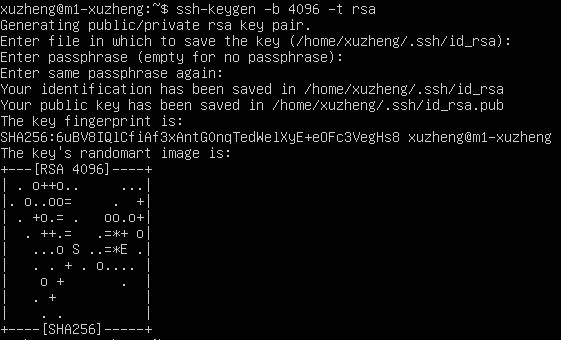
\includegraphics[width=7cm]{../images/13.png}
    \end{subfigure}%
    \begin{subfigure}{.5\textwidth}
        \centering
        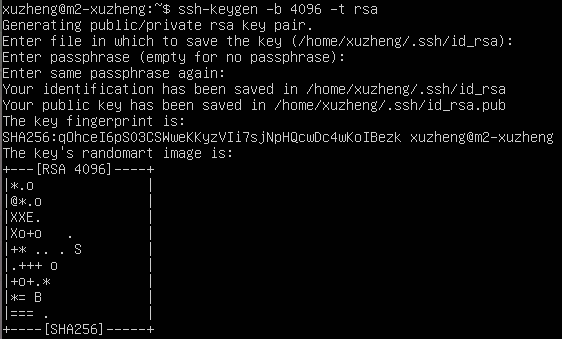
\includegraphics[width=7cm]{../images/14.png}
    \end{subfigure}
\end{figure}
Ahora en lugar de utilizar \textbf{ssh-copy-id} vamos a utilizar \textbf{scp} para copiar la clave pública de una máquina al archivo \textit{.ssh/authorized\textunderscore keys} de otra:
\image{12}{18}
Comprobamos conectando desde m1 a m2:
\image{10}{19}
Como podemos observar, no nos ha pedido la contraseña.

\section{Crontab}
Para que se sincronice el directorio \textit{/var/www} entre las dos máquinas en cada hora,  editamos el archivo \textit{/etc/crontab} como sigue:
\image{12}{20}
De forma que en el minuto 0 de cada hora se va a ejecutar \textbf{rsync}.
\subsection{Opciones avanzadas}
Aparte del \textbf{*} para indicar todos los valores, también podemos usar entre otras opciones: \textbf{-} para indicar el rango de tiempo y \textbf{/} para indicar el salto de tiempo. En el siguiente ejemplo, vamos a utilizar \textbf{crontab} para escribir la hora en un archivo en cada 90 minutos empezando por la media noche:
\image{12}{21}

\newpage
\section{Bibliografía}
\begin{itemize}
    \item \url{https://linux.die.net/man/1/scp}
    \item \url{https://linux.die.net/man/1/tar}
    \item \url{https://serverfault.com/questions/141773/what-is-archive-mode-in-rsync}
    \item \url{https://ss64.com/bash/rsync.html}
    \item \url{https://linux.die.net/man/1/rsync}
    \item \url{https://serverfault.com/questions/123629/run-task-every-90-minutes-with-cron}
\end{itemize}

\end{document}
